\documentclass{standalone}
\usepackage{tikz}
\usetikzlibrary{shapes}
\usetikzlibrary{positioning}
\usepackage{amsmath}


\begin{document}
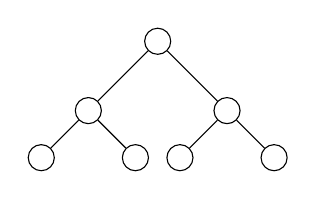
\begin{tikzpicture}[node distance=2cm]

    % \node(start)[startstop]{Start};
    \node(A)[draw, circle, minimum size=0.2cm]{};
    \node(B)[draw, circle, minimum size=0.2cm, below left=0.9cm of A]{};
    
    \node(D)[draw, circle, minimum size=0.2cm, below right=0.9cm of A]{};
    \node(F)[draw, circle, minimum size=0.2cm, below left=0.5cm of B]{};
    \node(G)[draw, circle, minimum size=0.2cm, below right=0.5cm of B]{};
    \node(E)[draw, circle, minimum size=0.2cm, below left =0.5cm of D]{};
    \node(C)[draw, circle, minimum size=0.2cm, below right=0.5cm of D]{};
    
    \draw (A) -- (B) -- (G);
    \draw (A) -- (D);
    \draw (B) -- (F);
    
    \draw (D) -- (E);
    \draw (D) -- (C);


\end{tikzpicture}
\end{document}
